% Reviewer (1)% Reviewer (2)% Reviewer (3)
\documentclass[10pt]{article}
\usepackage{a4wide}
\usepackage{xcolor}
\usepackage{color,soul}
\usepackage{mdframed}
\usepackage{caption}
\captionsetup[table]{skip=10pt}
\usepackage{enumerate}
\usepackage{url}
\usepackage{textcomp}
\newcommand{\rev}[1]{{\bf Rev.\,\##1}}
\newcommand{\latexdiff}{\texttt{latexdiff}}
\newcommand{\chk}[1]{\textcolor{red}{#1}}
\newcommand{\reviewer}[1]{\textbf{#1}}
\newcommand{\answer}[1]{#1}
\newcommand{\us}{\char`_}

\newcommand{\MT}[1]{\textcolor{blue}{MT: #1}}

\newcommand{\ccnsim}{ccn\ensuremath{\mathcal{S}}im} % \'a la rossini ;)
\newcommand{\akaroa}{Akaroa2\textcopyright\ }
\usepackage{textcomp}
\newcommand{\textapprox}{\raisebox{0.5ex}{\texttildelow}}

\newcommand{\firstfakeieeepar}[1]{\noindent{\textit{#1.}}}
\newcommand{\firstfakeacmpar}[1]{\noindent{\textbf{#1.}}}
\newcommand{\fakeieeepar}[1]{~\\\noindent{\textit{#1.}}}
\newcommand{\fakeacmpar}[1]{\vspace{2 mm}\noindent{\textbf{#1.}}}
\newcommand{\fakeacmparnobold}[1]{\noindent{\textit{#1.}}}
\newcommand{\fakesubsection}[1]{\fakeieeepar{#1}}
\newcommand{\firstfakesubsection}[1]{\firstfakeieeepar{#1}}

\usepackage{tikz}

\newcommand\encircle[1]{%
  \tikz[baseline=(X.base)] 
    \node (X) [draw, shape=circle, inner sep=0] {\strut #1};}


%\renewcommand{\ccnsim}{ccnSim}

%\DeclareRobustCommand{\hlg}[1]{{\sethlcolor{cyan!10}\hl{#1}}}
\newcommand{\colorboxg}[1]{{\colorbox{gray!20}{#1}}}

%========================================================================
%  to make missing refs really standout
%------------------------------------------------------------------------
% http://www.latex-community.org/forum/viewtopic.php?f=5&t=13654
 \newcommand*{\missingreference}{\colorbox{red}{?reference?}}
 \newcommand*{\missingcitation}{\colorbox{red}{?citation?}}
 \makeatletter
 \def\@setref#1#2#3{%
   \ifx#1\relax
    \protect\G@refundefinedtrue
    \nfss@text{\reset@font\missingreference}%
    \@latex@warning{Reference `#3' on page \thepage \space
              undefined}%
   \else
    \expandafter#2#1\null
   \fi}
 \def\@citex[#1]#2{\leavevmode
   \let\@citea\@empty
   \@cite{\@for\@citeb:=#2\do
    {\@citea\def\@citea{,\penalty\@m\ }%
     \edef\@citeb{\expandafter\@firstofone\@citeb\@empty}%
      \if@filesw\immediate\write\@auxout{\string\citation{\@citeb}}\fi
      \@ifundefined{b@\@citeb}{\hbox{\reset@font\missingcitation}%
       \G@refundefinedtrue
        \@latex@warning
          {Citation `\@citeb' on page \thepage \space undefined}}%
        {\@cite@ofmt{\csname b@\@citeb\endcsname}}}}{#1}}
 \makeatother 
%========================================================================
%  to make missing refs really standout
%------------------------------------------------------------------------



\begin{document}

{\centering 
	{\Large {\bf \ccnsim-Parallel}}\\
	{\large Installation and User Guide}\\[10pt]
}

This introductory guide provides the key steps for the installation of the newly released \ccnsim-Parallel~\cite{ccnSim}, along with a couple of sample use cases.
\ccnsim-Parallel integrates the single-threaded ModelGraft technique \cite{tortelli-comnet:17}, implemented in \ccnsim-v0.4, with a new approach for parallelization, thus (i) increasing performance, in terms of CPU execution time, by nearly two orders of magnitude with respect to \ccnsim-v0.4, and (ii) enabling the simulation of web-scale scenarios (i.e., with catalogs comprising $10^{12}$ contents) within reasonable CPU times and memory requirements.   
For a thorough description of the single-threaded ModelGraft technique please refer to \cite{tortelli-comnet:17}, while for more details on the background at the bases of \ccnsim-Parallel we point the reader to our technical report \cite{pMG_techRep}.

\section*{Theoretical Background}
From a \emph{theoretical viewpoint}, \ccnsim-Parallel is designed around an innovative technique for parallelizing the simulation of general cache networks, referred as \emph{catalog slicing}. 
One of the classic ways for parallelizing simulations is that of geographically splitting the network into non-overlapping regions, and then mapping their simulation to multiple cores (or threads); it is a well-investigated approach that generates a significant communication overhead due to ``message passing'', especially in cache networks where requests' propagation creates strong correlation between the state of neighboring cache nodes.
With the \emph{catalog slicing} technique, instead, each core \emph{independently} simulates the whole topology and the whole downscaled catalog (since we resort on the ModelGraft \emph{downscaling} technique~\cite{tortelli-comnet:17}), but only for a fraction of time, before sending aggregated information to the master node.

In particular, the instantiation of multiple and independent parallel threads is made possible thanks to Che's approximation~\cite{wang02jsac_hierarchical}, according to which in a network of Least Recently Used (LRU) caches, dynamics of different contents can be considered as both spatially and temporally independent; as a consequence, 
distinct threads can be assigned to different portions of the request process timeline, thus sizing the global simulation time for each thread according to the maximum number of available threads.
An elected \emph{master} thread, then, will simply collect and sum statistics obtained by the different \emph{slaves} in order to compute the global network state and decide on both \emph{dynamic transient state} and \emph{simulation end}. 
This approach 
(i) avoids heavy communication overhead related to message passing, leading to a \emph{nearly proportional} gain with the number of parallel threads (up to \textapprox32 threads), and 
(ii) introduces and additional speedup with respect to the single-threaded ModelGraft~\cite{tortelli-comnet:17} of about \emph{2 orders of magnitude}. 
For a thorough evaluation of the new ModelGraft technique with parallelization, please refer to our technical report available at \cite{pMG_techRep}.     

\section*{Design Summary}
The design of \ccnsim-Parallel has involved the integration of two different softwares: 
(i) the open source \ccnsim-v0.4 simulator \cite{ccnSim}, which includes the implementation of the single-threaded ModelGraft technique, and 
(ii) the licensed \akaroa software~\cite{ewing:99,AkaroaPrj}, which provides APIs for the design of a master-slave infrastructure. 
Modifications have been made to both, in order to ease their integration, and adapt the code of \ccnsim\ to the \emph{parallel} ModelGraft technique, thus conceiving a unique and dedicated version, i.e., \ccnsim-Parallel, which is freely available at \cite{ccnSim}. 
Due to the strong integration between the two aforementioned softwares, \ccnsim-Parallel requires the modified \akaroa.
It is important to notice that users \emph{should obtain a specific license} for the download of the original Akaroa-2.7.13, i.e., the initial version used for the deployment of \ccnsim-Parallel; a specific \emph{patch}, instead, is freely distributed at \cite{ccnSim}, in order to integrate the required modifications.


\section*{Installation}
In this section we will cover all the steps needed for the installation of \ccnsim-Parallel. We suggest the reader to check and execute them by following the presentation order.

\subsection*{Portability}

\ccnsim-Parallel has been tested on the following platforms, and with the following softwares:
\begin{itemize}
     \item Ubuntu Linux 14.04 (64-bit)
     \item Ubuntu Linux 16.04 Server (64-bit)
     \item Omnetpp-4.6 
     \item Omnetpp-5.0 
     \item Akaroa-2.7.13 
\end{itemize}

\subsection*{Prerequisites}

 \begin{itemize}
     \item \textbf{Boost libraries $\ge$ 1.54}: they can be installed either by using the standard packet manager of your system (e.g., apt-get install, yum install, port install, etc.), or by downloading them from \url{http://www.boost.org/users/download/}, and following instructions therein.

     \item \textbf{gcc $>$ 4.8.1}: on Ubuntu platforms, gcc can be updated by adding the \colorboxg{ubuntu-toolchain-r/test} PPA. Sample commands for the latest 5.x version are: \\ 

     \ \ \colorboxg{sudo add-apt-repository ppa:ubuntu-toolchain-r/test} 

     \ \ \colorboxg{sudo apt update} 

     \ \ \colorboxg{sudo apt install gcc-5 g++-5} 
     
     \ \ \colorboxg{sudo update-alternatives -{}-install /usr/bin/gcc gcc /usr/bin/gcc-5 60}

     \ \ \ \ \ \ \ \ \ \ \ \ \colorboxg{-{}-slave /usr/bin/g++ g++ /usr/bin/g++-5}  \\

     \item \textbf{parallel-ssh}: in order to ease the simulation workflow, a passwordless SSH login needs to be present on all the available servers. \emph{parallel-ssh} can than be used in order to send commands to slaves from the master node. \\

     \ \ \colorboxg{sudo apt-get install pssh} 
\end{itemize}

\subsection*{\akaroa}
As mentioned above, \akaroa requires a specific license in order to be used. 
For instructions about software download and licenses, please visit the website \url{https://akaroa.canterbury.ac.nz/akaroa/}.
The design of \ccnsim-Parallel, concerning the Akaroa component, has started from the Akaroa-2.7.13 version. 
The whole set of modifications that have been made in order to implement the parallel ModelGraft strategy are grouped inside the \emph{Akaroa\_2.7.13\_for\_PMG.patch} patch, which is freely available at \url{http://perso.telecom-paristech.fr/~drossi/ccnSim}.

Once obtained the original licensed Akaroa-2.7.13, place it in the same directory with the aforementioned patch, and type: \\

\ \ \colorboxg{patch -s -p0 $<$ Akaroa\_2.7.13\_for\_PMG.patch} \\

Notice that the original Akaroa directory will keep the same name even after the application of the patch.

Once the patch is applied, type the following commands from the root directory of the patched Akaroa in order to install it: \\

\ \ \colorboxg{./configure} 

\ \ \colorboxg{make} 

\ \ \colorboxg{sudo make install} \\

Akaroa binaries, libraries, and include files will be installed in /usr/local/akaroa/bin, /usr/local/akaroa/lib, and /usr/local/akaroa/include, respectively.
If you \emph{do not have sudo privileges}, and you need to install Akaroa into another location, e.g., $<$install\_path$>$, please add this location to your PATH variable, and use the following commands: \\

\ \ \colorboxg{./configure -{}-prefix=$<$install\_path$>$} 

\ \ \colorboxg{make} 

\ \ \colorboxg{make install} \\

Furthermore, always in the case of lacking sudo privileges, users might need to modify LIB and PYTHON paths in the several ``Makefile.config\_*'' files and inside the ``pyconfig.py'' file according to the customized locations of related libraries, before compiling and installing Akaroa.


\subsection*{Omnet++}
\ccnsim-Parallel has been tested with both \emph{Omnetpp-4.6} and \emph{Omnetpp-5.0}, which are available at \url{https://omnetpp.org/}. 
Before the installation, Omnetpp-x requires prerequisite packages to be installed. For the complete list, please read the official installation manual. 
Furthermore, since Omnetpp-x bin/ directory needs to be added to the PATH variable, the following line should be put at the end of the \colorboxg{\textapprox/.bashrc} file: \\ 

\ \ \colorboxg{export PATH=\$PATH:\$HOME/omnetpp-x/bin} \\

After having closed and saved the file, please close and re-open the terminal.

\noindent Regardless of the Omnetpp version, a couple of patch files need to be applied to it before compilation and installation. 
These patch files are provided with \ccnsim-Parallel, which we suppose being correctly downloaded (see next section) and decompressed in the \$CCNSIM\_DIR.
Provided that Omnetpp is present in the \$OMNET\_DIR, specific instructions to patch, compile, and install it without the graphical interface (not needed for parallel ModelGraft simulations) are provided in the following, according to the selected version:

\begin{itemize}
     \item Omnetpp-4.6

     \ \ \colorboxg{pint:\textapprox\$ cd \$CCNSIM\_DIR} 

     \ \ \colorboxg{pint:CCNSIM\_DIR\$ cp ./patch/omnet\-4x/ctopology.h \$OMNET\_DIR/include/}

     \ \ \colorboxg{pint:CCNSIM\_DIR\$ cp ./patch/omnet\-4x/ctopology.cc \$OMNET\_DIR/src/sim/}

     \ \ \colorboxg{pint:CCNSIM\_DIR\$ cd \$OMNET\_DIR/}

     \ \ \colorboxg{pint:OMNET\_DIR\$ NO\_TCL$=$1 ./configure}

     \ \ \colorboxg{pint:OMNET\_DIR\$ make}


     \item Omnetpp-5.0

     \ \ \colorboxg{pint:\textapprox\$ cd \$CCNSIM\_DIR}

     \ \ \colorboxg{pint:CCNSIM\_DIR\$cp ./patch/omnet\-5x/ctopology.h \$OMNET\_DIR/include/omnetpp}

     \ \ \colorboxg{pint:CCNSIM\_DIR\$cp ./patch/omnet\-5x/ctopology.cc \$OMNET\_DIR/src/sim}

     \ \ \colorboxg{pint:CCNSIM\_DIR\$ cd \$OMNET\_DIR/}

     \ \ \colorboxg{pint:OMNET\_DIR\$ ./configure WITH\_TKENV$=$no }

     \ \ \colorboxg{pint:OMNET\_DIR\$ make}
\end{itemize}

Compilation flags can also be set through the file \emph{configure.user} (e.g., to disable Qtenv).

\subsection*{\ccnsim-Parallel}

As anticipated above, the .tgz file containing the \ccnsim-Parallel code can be obtained from \url{http://perso.telecom-paristech.fr/~drossi/ccnSim}.
After having decompressed it in the \$CCNSIM\_DIR folder, installation requires the following steps: \\

\ \ \colorboxg{./scripts/makemake.sh}

\ \ \colorboxg{make} \\

If all the steps described in the previous sections have been successfully executed, simulations of general cache networks using the parallel ModelGraft technique can now be launched. The several steps needed to simulate sample scenarios will be described in the following.

\section*{Example-1: ``Trillion'' made possible!}
In this section we will describe all the steps needed to simulate a Web-scale scenario, i.e., comprising a catalog with a trillion contents. It is an extreme scenario which highlights the capabilities of the new parallel ModelGraft technique. For an extended and thorough performance evaluation, which considers scenarios with different cardinalities, we refer the reader to our technical report \cite{pMG_techRep}. 

\subsection*{Scenario, bare-metal, and scripts}
\fakeacmpar{Scenario} We consider a CDN-like topology composed of an Abilene core network, and several 4-level binary trees attached to it, thus representing access networks. 
By using the resulted topology, which comprises 67 nodes in total, we simulate an initial non-downscaled catalog of $M=10^{12}$ contents, and through an Independent Reference Model (IRM), i.e., i.i.d. requests, we consider $R=10^{12}$ total requests as a non-downscaled initial point. 
We consider nodes having non-downscaled Least Recently Used (LRU) caches of $C=10^{8}$ contents.
By following guidelines provided in \cite{tortelli-comnet:17}, we set the \emph{downscaling} factor of the ModelGraft technique at $\Delta=10^7$. 
As a consequence, we effectively simulate a \emph{downscaled} catalog of $M'=10^5$ contents, with Time-to-Live (TTL) caches with a downscaled cache size of $C'=10$, and we generate a downscaled number of $R'=10^7$ requests.  

\fakeacmpar{Bare-metal} The dedicated cluster used for the experiment comprises $NS = 3$ Cisco UCS-B series servers, each one hosting 2 NUMA nodes, with a Xeon E5-2690 CPU, $NC = 12$ physical cores per NUMA node (i.e., 48 CPUs in total with hyperthreading) operating at 2.60GHz, and 378 GB of RAM memory.
For ease of description we call our servers ``modelgraftX'', where $X \in \{1,2,3\}$, and we suppose that a \emph{modelgraft} user is present in each of them. 
We also remind that it is important to have a passwordless SSH login on all the available servers. For this particular scenario, we report results related to simulations done with $NT = 64$ parallel threads and $NS = 2$ physical servers. 

\fakeacmpar{Scripts} The main file used to launch the simulation of the described scenario is: \\

\ \ \colorboxg{\encircle{1} ./launch\_Parallel\_ModelGraft\_1e12.sh} \\

This \emph{bash script} will appear inside the Akaroa folder after having applied the provided \\ Akaroa\_2.7.13\_for\_PMG.patch patch.
In order to make it executable you need to type \\
\colorboxg{chmod +x launch\_Parallel\_ModelGraft\_1e12.sh}.  
It is important to notice that:
\begin{itemize} 
\item The script is supposed to be executed from one of the servers used for the simulation, meaning that both Akaroa and \ccnsim-Parallel are installed on the same machine. If executed from a different machine than the servers used for the simulations, the script will need some modifications.
\item The script has been conceived considering the specified pool of 3 servers, i.e., modelgraft1, modelgraft2, and modelgraft3, with a common ``modelgraft'' user present on all of them;  
\item If using different servers and username, the script needs to be modified accordingly. Sometimes it is more practical to use server names instead of IP addresses; in order to do that, entries like "x.x.x.x servername" should be added in the ``/etc/hosts'' file of all the servers.
\end{itemize}

\emph{We strongly suggest to carefully read both the extensively documented script \encircle{1} for a detailed description of all its components and commands, and the User Manual of \ccnsim-v0.4 \cite{ccnSim} for insights related to its structure and to the ModelGraft technique}. \\
In summary, script \encircle{1} will:

\begin{enumerate}[I.]

\item specify the number of \emph{physical servers} and \emph{parallel threads} that will be used to run the parallel ModelGraft;

\item set all the parameters needed to define the simulated scenario;

\item automatically probe and allocate resources on the available servers according to their load (i.e., the least loaded ones are considered);

\item launch Akaroa daemons (both Master and Slaves) on the reserved resources; \\

\ \ \colorboxg{\$\{akaroaBinDir\}/akmaster \&}

\ \ \colorboxg{\$\{akaroaBinDir\}/akslave \&}

\item call the script ``runsim\_script\_Parallel\_ModelGraft.sh'' dedicated to \ccnsim-Parallel simulations. 

\end{enumerate}
\vspace{8mm}
\ \ \ \ \colorboxg{\encircle{2} ./runsim\_script\_Parallel\_ModelGraft.sh \{parameters\}} \\

All the scenario parameters defined within script \encircle{1} are passed in the form of command line parameters to script \encircle{2}, which is located in \$CCNSIM\_DIR. For a complete list of all the possible {parameters} please refer to the User Manual of \ccnsim-v0.4 \cite{ccnSim}.

\emph{We strongly suggest to carefully read the extensively documented script \encircle{2} for a detailed description of all its components and commands, and the User Manual of \ccnsim-v0.4 \cite{ccnSim} for insights related to its structure and to the ModelGraft technique}. \\
In summary, script \encircle{2} will:

\begin{enumerate}[I.]

\item  check if the required $T_C$ file is already available; otherwise it will create a new one with \emph{random} $T_C$ values, which will be distributed to all the available servers;

\item  create a new .ini file according to \{parameters\};

\item  launch the parallel ModelGraft simulations through the Akaroa APIs;

\item  collect and elaborate results. 

\end{enumerate}

Point I. is worth to be discussed: since the ModelGraft technique \cite{tortelli-comnet:17} makes use of TTL caches with an eviction timer set according to the \emph{characteristic time} $T_C$ \cite{wang02jsac_hierarchical} of the respective LRU caches, files reporting the $T_C$ value of each node in the simulated topology are needed as input.
Since in most of the real scenario users do not know $T_C$ values a priori, the ModelGraft technique is able to iteratively converge to a consistent state through a feedback loop, even when accepting random $T_C$ values as input. As a consequence, script \encircle{2} will firstly check if a user-provided $T_C$ file is already present, and if not, it will randomly generate values for all the nodes, collect them in one file, and distribute it to all the available servers (since all the threads instantiated over multiple servers need to have a common $T_C$ file as a starting point). This file will be automatically erased from all the servers if randomly generated (i.e., user-defined ones will not be erased).  

As for the management of the output files produced by all the parallel threads, the policy adopted by the current version of script \encircle{2} is that of \emph{removing them all from each server, thus saving only a SUMMARY file}, namely ``ALL\_MEASURES*'', which will be kept in the \\ \emph{\$\{CCNSIM\_DIR\}/\$\{resultDir\}/parallel} folder of the server where script \encircle{2} has been executed from (which, by default, is modelgraft1). 
If you want/need to change this policy, please follow instructions provided in the script \encircle{2} file.


\subsection*{Results}
Results are presented in Fig. \ref{fig:cpu_mem_1e12}, which reports both CPU time and memory occupancy on a logarithmic axis; in particular, results related to three different strategies are compared: classic event-driven (ED) simulation, single-thread ModelGraft, and the last parallel ModelGraft technique. 
As it can be noticed, simulating such a huge scenario would be prohibitive if relying on the classic event-driven approach, considering that we would need more than one year of CPU time and more the 7 TBytes of RAM. That is the reason why we report only projected results, computed from linearly interpolating results obtained for smaller scenarios. Since the introduction of the single-threaded ModelGraft technique \cite{tortelli-comnet:17}, instead, memory occupancy is not considered as a bottleneck anymore (notice that only 27 MB are required); as a consequence, CPU time represented the only bottleneck (i.e., for this scenario, we would need more than 2 days of simulation). 
The new parallel ModelGraft technique, indeed, aims at overcoming the CPU bottleneck by parallelizing the simulation over multiple threads and physical servers. In this particular case, by instantiating $NT=64$ parallel threads over $NS=2$ physical servers, we notice from Fig. \ref{fig:cpu_mem_1e12} a dramatic decrease in the CPU time, i.e., 9056$\times$ and 42$\times$ compared to classic ED simulation and single-threaded ModelGraft, respectively. As for the memory occupancy, instead, we can observe that while parallelizing the simulation by creating exact replicas of network and catalog increases the required memory, the total amount is still considerably slow and it can also be split over multiple servers. At the same time, the parallel ModelGraft technique still considerably reduces the memory occupancy w.r.t. ED simulation by up to 4065$\times$. 


\section*{Example-2: Parallel MG vs MG vs Classic ED Simulation}
The Web-scale scenario seen before is treatable only by using the scalability and performance of the parallel ModelGraft technique, meaning that we actually miss other points of comparison. As a consequence, in this section we compare the new parallel ModelGraft technique against the previous single-threaded one, and against the classic event-driven (ED) simulation (both available with \ccnsim-v0.4 \cite{ccnSim}), by considering a smaller scenario as a reference. 

In particular we simulate a 4-level binary tree (i.e., 15 nodes) topology, with a non-downscaled catalog cardinality of $M=10^9$, cache size $C=10^6$, $R=10^9$ total requests, and a downscaling factor of $\Delta=10^5$. This scenario can be simulated by using the provided script \\
\ \ \colorboxg{./launch\_Parallel\_ModelGraft\_1e9.sh} 

\begin{figure}[t] 
  \centering
    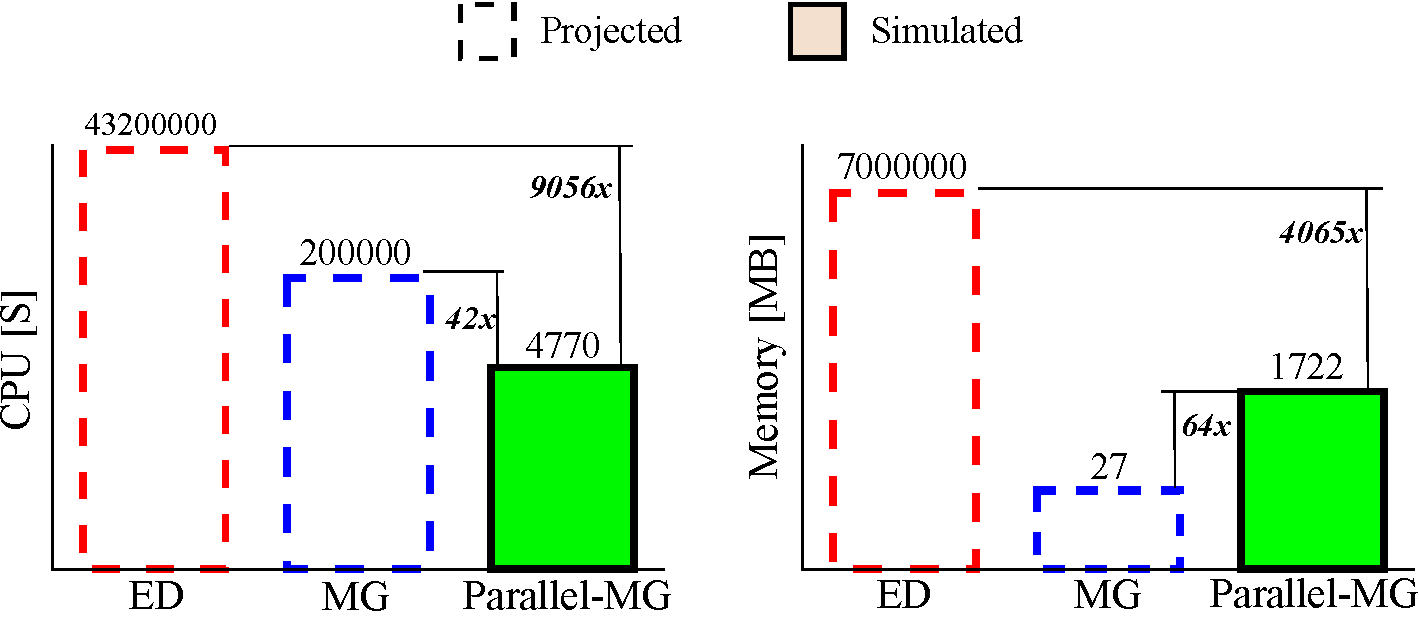
\includegraphics[width=0.9\textwidth]{plot_cpu_mem_1e12_NEW.pdf}
  \caption{Parallel ModelGraft vs ED and ModelGraft projections: CPU time and Memory occupancy for Web-scale scenario ($M=10^{12}$, $R=10^{12}$, $C=10^8$, $\Delta=10^7$, $NT=64$ parallel threads, $NS=2$ physical servers for the parallel ModelGraft technique).}
  \label{fig:cpu_mem_1e12}
\end{figure}

\subsection*{Results}
Results reported in Tab. \ref{tab:table_1e9} highlight three main considerations: (i) the parallelization of the ModelGraft technique \emph{does not introduce further inaccuracies}, it (ii) allows to \emph{drastically reduce the CPU time} of a further order of magnitude with respect to the single-threaded ModelGraft, while (iii) still \emph{requiring a reasonable amount of memory} with respect to the number of instantiated parallel threads, i.e., 32 in this case (it is worth considering that the total memory demand can be spread over multiple machines when multiple servers are available).   


\section*{Customization}

\subsection*{General Information} 
Users interested in experimenting and ameliorating the implementation of the parallel ModelGraft technique can refer to the CHANGELOG.txt file (present in both patched Akaroa folder and \ccnsim-Parallel folder) where a list enumerating all the modified files is reported. The goal is that of facilitating the orientation of newcomers into both Akaroa and \ccnsim-Parallel codebases. 
Nevertheless, for a deeper understanding of all the elements included in the parallel ModelGraft technique, we strongly encourage users to read (i) Akaroa documentation \cite{AkaroaPrj}, \ccnsim-v0.4 documentation \cite{ccnSim}, ModelGraft paper \cite{tortelli-comnet:17}, the parallel ModelGraft technical report \cite{pMG_techRep}, and all the well documented scripts present in both patched Akaroa folder and \ccnsim-Parallel folder.

\subsection*{Applicability}
For a complete list and discussion on all the possible scenarios the parallel ModelGraft technique can be used for, please refer to Section 3.1 of the \ccnsim-v0.4 manual \cite{ccnSim}.  

\subsection*{Encoding of Messages Exchanged between Master and Slaves}
The patched Akaroa-2.7.13 needs to define a MAX\_MSG\_LENGTH variable for the messages which are exchanged between Master and Slaves. 
In addition, one of the modifications introduced in order to let Akaroa and ccnSim-Parallel communicate and be compliant with each other, is that of including a \emph{vector}, namely ``HitMissVector'', inside the exchanged messages. This vector should contain info about hit and miss events collected by the parallel and independent slaves, which are then sent to the Master node. 

\begin{table}[t] 
  \centering
  \caption{Parallel ModelGraft vs ModelGraft vs Event-driven simulation: accuracy loss, CPU and memory gain for a very large scenario ($M=10^{9}$, $R=10^{9}$, $C=10^6$, $\Delta=10^5$, $NT=32$ parallel threads, $NS=1$ physical server for the parallel ModelGraft technique)}\label{tab:table_1e9}
    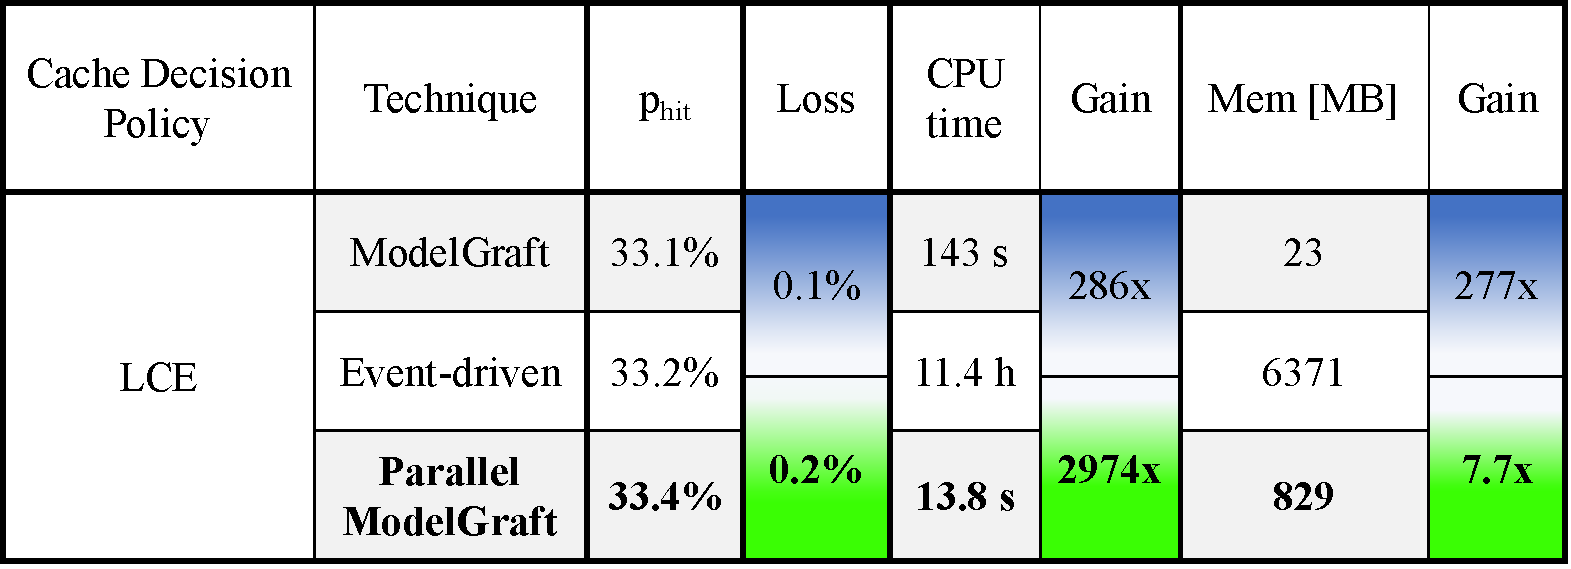
\includegraphics[width=0.9\textwidth]{table_1e9.pdf}
\end{table} 

For the ease of implementation, both MAX\_MSG\_LENGTH and HitMissVect have been sized according to the biggest simulated topology. In practice, since each node in the network will send $2 \times engineWindow = 2 \times (W/NT)$ Hit and Miss samples, where $W$ is the initially dimensioned window size, and $NT$ is the number of allocated parallel threads, the size of the \emph{aggregated} HitMissVect sent by each parallel thread will be equal to  $vectSize = N \times 2 \times engineWindow$, where $N$ is the total number of nodes. 
Since $W=100$ by default, and since the largest topology that we simulated is the CDN-like one (i.e., with 67 nodes), the aforementioned variables are set at compile time as: \\

\ \ char HitMissVect[57000] (inside `src/include/checkpoint.H' file of Akaroa)

\ \ \#define MAX\_MSG\_LEN 57500 (inside src/ipc/connection.H' file of Akaroa) \\

The HitMissVect size (in Bytes) has been obtained by $N \times 2 \times engineWindow \times 4$, supposing $NT=1$ (i.e., the case with the biggest vector). 
The exact value should be 53600 Bytes, so the used one is slightly increased for safety reasons.
The size of the MSGs that should carry also the HitMissVect is, then, set accordingly to $MAX\_MSG\_LEN=57500$ (i.e., 500 Bytes more to reserve space for other values transmitted within the same message).

It is IMPORTANT to notice that, if using other values then $N=67$, $W=100$, which bring to a bigger HitMissVect than 57000 Bytes (the equation is always $N \times 2 \times (W/NT)$), please modify the relative \emph{checkpoint.H} and \emph{connection.H} files, and recompile Akaroa (make; sudo make install). 
If smaller values are set w.r.t. the real ones, segmentation fault problems might happen.  



\bibliographystyle{plain}
\bibliography{biblio}



\end{document}
